
% =============================================================================
% introduction
% =============================================================================

\chapter{Introduction}

%Here put a general but short introduction to the needs of standardizing the representation of pathways.
With the rise of systems and synthetic biology, the use of graphical representations of pathways and networks to describe biological systems has become pervasive. It was therefore important to use a consistent notation that would allow people to interpret those maps easily and quickly, without the need of extensive legends. Furthermore, activities like synthetic biology, that reconstruct biological systems, need to exchange their descriptions unambiguously, as engineers exchange circuit diagrams. 

The goal of the Systems Biology Graphical Notation (SBGN) is to standardize the graphical/visual representation of biochemical and cellular processes. SBGN defines comprehensive sets of symbols with precise semantics, together with detailed syntactic rules defining their use.  
It also describes the manner in which such graphical information should be interpreted. SBGN is made up of three different and complementary languages \cite{LeNovere:2009p1}. This document presents the graphical elements composing the \emph{\PDl{}} of SBGN. It is not a normative description, but rather a document aimed at end users. People, such as software developers, looking for a normative description of SBGN \PDs should rather read the technical specification of the language \cite{Moodie:2011}.

\section{Overview of SBGN \PDs}
\label{sec:PD-overview}

To quickly describe what SBGN \PDl is about, let's give a brief overview of some of the relevant concepts with the help of an example shown in \fig{eg1}. It is a simple map for part of a mitogen-activated protein kinase (MAPK) cascade.  The larger nodes in the figure (some of which are in the shape of rounded rectangles and others in the shape of circles) represent biological materials---things like macromolecules and simple chemicals (NB: the nodes representing physical entities (or proxies to physical entities) will always be colored in yellow in this document. Color is not part of the SBGN specification though). The biological materials are altered via processes (colored in green in this document), which are indicated in \PDl by lines with arrows and other decorations.  In this particular map, all of the processes happen to be the same: processes catalyzed by biochemical entities.   
The directions of the arrows indicate the direction of the processes; for example, unphosphorylated RAF kinase proceeds to phosphorylated RAF kinase via a process catalyzed by RAS. Although ATP and ADP are shown as incidental to the phosphorylations on this particular graph, they are involved in the same process as the proteins getting 
phosphorylated. The small circles on the nodes for RAF and other entity pools represent state variables (in this case, phosphorylation sites). 

% Redo the figure with colors
\begin{figure}[h]
  \centering
  \vspace*{-0.75em}
  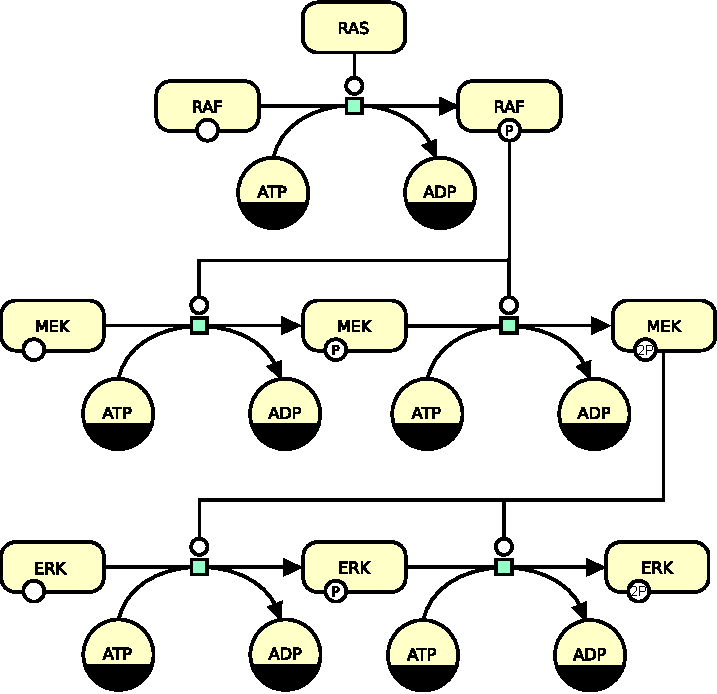
\includegraphics[scale=0.8]{images/MAPK-only}
  \caption{This example of a \PD uses two kinds of entity pool nodes: one for pools of different macromolecules (\sect{macromolecule}) and another for pools of simple chemicals (\sect{simpleChemical}). Most macromolecule nodes in this map are adorned with state variables (\sect{stateVariable}) representing phosphorylation states. This map uses one type of process node, the process node (\sect{process}), and three kind of connecting arc, consumption (\sect{consumption}), production (\sect{production}) and catalysis (\sect{catalysis}).  Finally, some entity pool nodes have dark bands along their bottoms; these are clone markers (\sect{cloneMarker}) indicating that the same pool nodes appear multiple times in the map.}
  \label{fig:eg1}
\end{figure}

The essence of the \PDs is \emph{change}: it shows how different entities in the system process from one form to another.  The entities themselves can be many different things.  In the example of \fig{eg1}, they are either pools of macromolecules or pools of simple chemicals, but as will become clear later in this chapter, they can be other conceptual and material constructs as well.  Note also that we speak of \emph{entity pools} rather than individuals; this is because in biochemical network models, one does not focus on single molecules, but rather collections of molecules of the same kind.  The molecules in a given pool are considered indistinguishable from each other.  The way in which one type of entity is transformed into another is conveyed by a \emph{process node} and arcs between entity pool nodes and process nodes indicate an influence by the entities on the processes.  In the case of \fig{eg1}, those arcs describe consumption \sect{consumption}, production \sect{production} and catalysis 
\sect{catalysis}, but others are possible.  Finally, nodes in \PDs are usually not repeated; if they do need to be repeated, they are marked with \emph{clone markers}---specific modifications to the appearance of the node (\sect{cloneMarker}). The details of this and other aspects of \PD notation are explained in the rest of this chapter.

\section{SBGN levels and versions}
\label{sec:sbgn-levels}

It was clear at the outset of SBGN development that it would be impossible to design a perfect and complete notation right from the beginning.  Apart from the prescience this would require (which, sadly, none of the authors possess), it also would likely need a vast language that most newcomers would shun as being too complex.  Thus, the SBGN community followed an idea used in the development of other standards, i.e. stratify language development into levels.

A \emph{level} of one of the SBGN languages represents a set of features deemed to fit together cohesively, constituting a usable set of functionality that the user community agrees is sufficient for a reasonable set of tasks and goals.  Within \emph{levels}, \emph{versions} represent small evolution of a language, that may involve new glyphs, refined semantics, but no fundamental change of the way maps are to be generated and interpreted. In addition new versions should be backwards compatible, \ie \PD maps that conform to an earlier version of the \PDl within the same level should still be valid.  This does not apply to a new levels. 

Capabilities and features that cannot be agreed upon and are judged insufficiently critical to require inclusion in a given level, are postponed to a higher level or version.  In this way, the development of SBGN languages is envisioned to proceed in stages, with each higher levels adding richness compared to the levels below it.

\section{How to get more information}
\label{sec:info}

The normative description of the language is the technical specification \cite{Moodie:2011}. It is available from the SBGN website (\url{http://sbgn.org/}). This website is a portal for all things to the notation. In addition to the specifications, there are examples of maps, FAQs, and informations on part and forthcoming meetings.  

The easiest and best way to get involved in SBGN  discussions is to join the sbgn-discuss@caltech.edu mailing list. If you only want the announcements of meetings and new specifications, you can join the very low flux mailing list sbgn-announce@lists.sf.net instead.
